\documentclass[compsoc, a4paper]{IEEEtran}

% Include packages
\usepackage[T1]{fontenc}
\usepackage[utf8]{inputenc}
\usepackage[inline]{enumitem}
\usepackage{acro, csquotes, amsmath, microtype, tikz, pgfplots, hyperref, inconsolata, bm, amssymb, siunitx, algpseudocode, fixme, mathtools, booktabs, siunitx, algorithmicx, algpseudocode, enumitem}
\usepackage[caption = false, labelfont = sf, textfont = sf]{subfig}
\usepackage[nocompress]{cite}

% Package setups
\setenumerate{label = (\alph*)}
\usetikzlibrary{positioning, arrows.meta}
\tikzset{
  every label/.style = { fill = white, inner sep = 1pt },
  every node/.style = { label distance = 2pt },
  arrow/.style = { ->, > = stealth, semithick, shorten > = 2pt, shorten < = 2pt }
}
\fxsetup{draft, layout = margin, author =, marginface = \scriptsize, inlineface = \scriptsize}
\hypersetup{hidelinks}
\pgfplotsset{compat=1.16}
\sisetup{detect-all}
\acsetup{short-format = \uppercase}

% Acronyms
\DeclareAcronym{kb}{short = kb, long = knowledge base}
\DeclareAcronym{yago}{short = yago, long = yet another great ontology}
\DeclareAcronym{kg}{short = kg, long = knowledge graph}
\DeclareAcronym{hake}{short = hake, long = hierarchy-aware knowledge graph embedding}
\DeclareAcronym{mrr}{short = mrr, long = mean reciprocal rank}
\DeclareAcronym{han}{short = h@n, long = hits-at-$n$}

% Custom "theorom" environments
\newtheorem{definition}{Definition}
\newtheorem{example}{Example}

\title{Link Prediction in Knowledge Graphs Using Graph Embedding}
\author{Emil S. Bækdahl \\ \url{ebakda16@student.aau.dk} \\ Group d806f20}

\begin{document}

\maketitle
\begin{abstract}
  \Aclp{kb} are becoming increasingly popular in both academia and industry since they provide an intuitive way to reason about data and thus can support decision making.
  Recently, an interest in inferring new knowledge from existing \aclp{kb} has seen a rise.
  For instance, in the medical domain, inference can be used to propose new drugs or treatments for known diseases.
  In this project, we examine a state-of-the-art approach to this problem that uses graph embeddings to predict missing links in \aclp{kb}.
  Particularly, we focus on a recent approach called the \acl{hake} and evaluate its performance on existing and new datasets.
  As a conclusion, we are not able to reproduce the results of the associated paper, and experiments on a new domain-specific dataset exhibit significantly poor performance.
\end{abstract}

\acresetall%

\section{Introduction}\label{sec:introduction}

Representation of knowledge in a way that suits computation is at the core of many machine intelligence tasks and agents.
A collection of such knowledge is called a \ac{kb} and it describes how different entities in a domain are related.
A \ac{kb} can be constructed either manually or automatically by computer programs that extract knowledge from existing sources.
Either way, during the construction, there might be a trade-off between completeness and correctness\cite{Paulheim2016}.
Completeness describes how well a \ac{kb} captures all knowledge in the desired domain while correctness describes the degree of truth of the knowledge.
When creating a \ac{kb} by hand, it is possible to manually verify the correctness of the knowledge.
However, it can be an infeasible task to manually cover all knowledge in larger domains, resulting in an incomplete \ac{kb}.
To speed up this process, automatic methods, such as building computer programs that extract knowledge, can be used.
However, while automatically extracting knowledge from many different sources can give a complete \ac{kb}, it may result in creating false knowledge.
The trade-off lies in finding a reasonable balance between correct and complete knowledge.

As a consequence of this issue, it is attractive to develop solutions that improve correctness or completeness of \acp{kb}.
This task is called \ac{kb} refinement and approaches to it are either concerned with
\begin{enumerate*}
  \item increasing completeness by inferring new or hidden knowledge from existing knowledge, or
  \item increasing correctness by finding and removing false knowledge.
\end{enumerate*}
Especially the former sees a gain in popularity since it can provide otherwise undiscovered insight into existing data and thus help humans in decision making.

One approach to computationally increasing completeness is through link prediction.
The goal of this task is to infer new knowledge by identifying missing links between existing entities in a \ac{kb}.
For link prediction, the current most popular methods are based on vector embeddings of \acp{kb}.
In this project, we take a closer look at this state-of-the-art technique.
Specifically, we focus on a recent technique that uses a \ac{hake} of \acp{kb} to infer missing links between entities in a hierarchical graph structure\cite{Zhang2019}.
We explain the underlying concepts for this technique and conduct experiments with existing datasets and a new domain-specific dataset.

The rest of this report is structured as follows.
Section~\ref{sec:related-work} discusses existing work on \acp{kb} and techniques for graph embedding and link prediction.
In Section~\ref{sec:preliminaries}, we introduce preliminary concepts in the field which will be the foundation for understanding the \ac{hake} technique in Section~\ref{sec:method}.
Using the technique, we conduct experiments and present their results in Section~\ref{sec:experiments}.
In Section~\ref{sec:discussion}, we discus the results and highlight some key ideas that can point in directions of future work.
We end with a conclusion in Section~\ref{sec:conclusion}.

\section{Related Work}\label{sec:related-work}

In this section, we touch upon two categories of related work: \ac{kb} sources and link prediction techniques.

A number of freely available and open source \acp{kb}, created in different ways, are described in\cite{Paulheim2016}.
The two most notable that cover general knowledge are Wikidata and DBpedia.
Both represent the knowledge found in the online encyclopaedia Wikipedia, but they do it in two distinct ways.
Wikidata is the underlying provider of knowledge to Wikipedia with data curated by the community\cite{Vrandecic2014}.
On the other hand, DBpedia extracts knowledge directly from the web pages of Wikipedia based on their text content\cite{Lehmann2015}.

\Ac{yago}\cite{Suchanek2007} is a \ac{kb} similar to DBpedia in the sense that most of its knowledge is extracted from Wikipedia.
However, the semantic lexicon WordNet is used to resolve ambiguity problems and gives \ac{yago} better correctness.
Since \ac{yago} is based on data from multiple sources, it naturally contains more knowledge compared to DBpedia.
Moreover, Wikidata, DBpedia, and \ac{yago} rely on data that are already structured.
Other approaches to constructing \acp{kb} are more automatic and based on unstructured data, for instance NELL\cite{Carlson2010} and Knowledge Vault\cite{Dong2014}.

All of the mentioned \acp{kb} can be accessed in a document format, typically RDF.\@
Furthermore, Wikidata, DBpedia, and \ac{yago} provide a SPARQL service for remote querying.
In this project, we will use Wikidata to construct a domain-specific dataset for experiments since it contains the most up-to-date data and provides a stable SPARQL interface.

Approaches to the link prediction problem come in a variety of flavours.
Some of the simplest techniques are based on similarity between nodes in a graph representation of a \ac{kb}\cite{Lue2011}.
Here, the heuristic is that similar nodes are more likely to be linked.
The major challenge with these approaches is that similarity can be measured in many different ways.
In\cite{Lue2011} alone, more than 20 measures are described and the authors add that the performance of the different measures may vary from case to case.
As such, deciding on a good similarity measure is not a trivial task.
Other techniques approach link prediction as a matrix factorisation problem.
As an example, the RESCAL\cite{Nickel2011} method factorises a three-dimensional matrix representation of a \ac{kb} and produces a model that captures features of the data which can be used to predict missing links.

Many recent link prediction techniques are based on vector representations of \acp{kb}.
This representation is called a graph embedding and in the context of link prediction, it can be used in a number of ways.
Currently, one of the most popular ways to use graph embeddings for link prediction is in translational models.
In a translational model, knowledge about entities is represented as translations in the graph embedding.
One of the first link prediction methods based on this approach is TransE\cite{Bordes2013}.
TransE have since been extended by the RotatE method\cite{Sun2019} which is based on embeddings in a complex vector space.
Using this approach, RotatE has the ability to model complicated \ac{kb} relations which is not possible with TransE.
Recently, the RotatE method inspired the \ac{hake} technique\cite{Zhang2019} which is based on embeddings in a polar coordinate system.
The purpose of the method is to exploit the nature of polar coordinates to persist the hierarchical nature of knowledge.
The \ac{hake} technique currently produces state-of-the-art results in the link prediction task.

In this paper, we will take a closer look at the \ac{hake} technique by examining its underlying theory and replicating the experiments from the original paper.
We also test the technique further by applying it to a domain-specific \ac{kb} extracted from Wikidata.

\section{Preliminaries}\label{sec:preliminaries}

In the following, we cover a number of topics that lay the foundation for the \ac{hake} technique and how it is used for link prediction.
In Section~\ref{sec:knowledge-bases}, we introduce \acp{kb} at the conceptual level and describe a way of representing them as graphs.
Section~\ref{sec:embedding} focuses on graph embedding and how they can be used for link prediction

\subsection{Knowledge Bases}\label{sec:knowledge-bases}

A \acf{kb} is a collection of facts that explain how different concepts in a certain domain are related.
Throughout this project, we will use the medical domain for exemplification, however, \acp{kb} can also span multiple domains.
The constituents of a \ac{kb} are divided into two categories: entities and relations.
An entity can be a concrete object or an abstract concept.
In our case study, an example of an entity is a concrete drug such as aspirin, but it can also something more abstract such as the class of infectious diseases.
A relation describes a connection between two entities.
For instance, a relation can describe a medical treatment by linking a drug and a disease.
Together, entities and relations form facts.
Formally, we define a \ac{kb} in the following way.

\begin{definition}[\Acl{kb}]\label{def:kb}
  Given a set of entities $\mathcal{E}$ and a set of relations $\mathcal{R}$, a \acf{kb} is a set of triples $\mathcal{K} = \{(h, r, t) \mid h, t \in \mathcal{E} \wedge r \in \mathcal{R} \}$ where each triple is a fact describing a relation $r$ between a head entity $h$ and a tail entity $t$.
\end{definition}

\begin{example}[A simple \acl{kb}]\label{ex:kb}
  Suppose we want to represent the fact that pain can be treated with aspirin.
  For this we need two entities, \textsc{pain} and \textsc{aspirin}, and one relation, \textsc{treated with}.
  Together, these make up one fact in the \ac{kb} $\mathcal{K}$ which, based on Definition~\ref{def:kb}, can be formulated in the following way.
  \begin{align*}
    \mathcal{E} & = \{\textsc{pain}, \textsc{aspirin}\}                          \\
    \mathcal{R} & = \{\textsc{treated with}\}                                    \\
    \mathcal{K} & = \{(\textsc{pain}, \textsc{treated with}, \textsc{aspirin})\}
  \end{align*}
\end{example}

In order to defined the link prediction problem introduced in Section~\ref{sec:introduction}, we first define a more general problem.
Inference in \acp{kb} is concerned with the completeness aspect of \ac{kb} refinement and is defined in the following way.

\begin{definition}[\Acl{kb} inference]\label{def:kb-inference}
  Let $\mathcal{K}^*$ be a \ac{kb} of all true knowledge and $\mathcal{K}$ be a \ac{kb} of observed knowledge such that $\mathcal{K} \subset \mathcal{K}^*$.
  The problem of \ac{kb} inference is to compute the missing knowledge $\mathcal{K}'$ in $\mathcal{K}$ such that $\mathcal{K} \cup \mathcal{K}' = \mathcal{K}^*$.
\end{definition}

The term \enquote{missing knowledge} in Definition~\ref{def:kb-inference} can be refer to both relations and entities.
In the context of the medical domain, finding a missing relation between a disease and a drug can hint at a new treatment, while discovering missing entities can lead to new drug proposals.

To represent a \ac{kb}, we can use an edge-labelled directed graph where nodes represent entities and edges represent relations.
This graph-based representation is defined in the following.

\begin{definition}[\Acl{kg}]
  A \acf{kg} is a 3-tuple $(V, E, \phi)$ where $V$ is the set of entities, $E \subseteq V \times V$ is the set of relations, and the function $\phi \colon E \rightarrow \mathcal{T}$ assigns a relation $\mathcal{T}_i \in \mathcal{T}$ to each $e \in E$.
\end{definition}

The direction of a relation in a \ac{kg} is implied by the direction of its corresponding edge.
For instance, the arrow in \figurename~\ref{fig:one-fact-kb-graph}, which represents the \ac{kb} from Example~\ref{ex:kb}, indicates that pain is treated with aspirin and not the other way around.

\begin{figure}[ht]
  \centering\small
  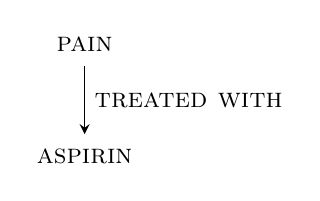
\begin{tikzpicture}
    \node (pain) {\scshape pain};
    \node (aspirin) [below = of pain] {\scshape aspirin};
    \draw [arrow] (pain) -- node[right] {\scshape treated with} (aspirin);
  \end{tikzpicture}
  \caption{The \ac{kb} $\mathcal{K} = \{(\textsc{pain}, \textsc{treated with}, \textsc{aspirin})\}$ represented as a \acl{kg}.}%
  \label{fig:one-fact-kb-graph}
\end{figure}

Any \ac{kb} $\mathcal{K}$ over entities $\mathcal{E}$ and relations $\mathcal{R}$ can be represented as a \ac{kg} by letting $V = \mathcal{E}$ and $E = \{(h, t) \mid (h, r, t) \in \mathcal{K}\}$.
The edge labelling function is defined such that $\phi(h, t) = r$ for each $(h, r, t) \in \mathcal{K}$.

Over recent years, \acp{kg} have become synonymous with \acp{kb} and is likely a more frequently used term.
Throughout this project, we use the term \ac{kg} as an interchange for \ac{kb}.
For example, we can talk about triples $(h, r, t)$, as defined in Definition~\ref{def:kb}, in the context of a graph.

Now that we have a concrete representation of knowledge in the form of a \ac{kg}, we can put the inference problem from Definition~\ref{def:kb-inference} into context and formulate the precise problem that we address in this project.

\begin{description}
  \item [\emph{Problem formulation}]
        Let $\mathcal{K} = (V, E, \phi)$ be a \ac{kg} where $E$ is the observed relations, or links, between the entities $V$.
        Let $E^*$ denote the set of all possible true links.
        Then the set $E' = E^* \setminus E$ represents the missing links in $\mathcal{K}$.
        The task of link prediction is to predict whether a given link $e \in V \times V$ such that $e \not\in E$ is true, i.e.\ if $e \in E^*$\cite{Li2018,Lue2011}.
\end{description}

The link prediction problem concerns the completeness aspect of \ac{kb} refinement, introduced in Section~\ref{sec:introduction}, with focus on identifying missing relations.
A solution to the problem typically consists of assigning a probability of existence to a potential edge in $V \times V$.
In the following section, we will dive deeper into graph embedding which is the foundation for many recent link prediction techniques.

\subsection{Graph Embedding}\label{sec:embedding}

To make graphs more efficient to work with computationally, it can be beneficial to embed them into a vector space\cite{Cai2018}.
This technique is called graph embedding.
The goal of graph embedding is to keep the dimensionality of the target vector space, called the embedding space, low while preserving properties of the graph.
Depending on the properties of interest, the embedding can happen on different levels.
For instance, in weighted graphs, each edge $e$ between two nodes $u$ and $v$ is associated with a weight $w(e)$ that can be used to represent, for instance, the importance or capacity of $e$.
This weight can be represented in the embedding by letting the distance between $u$ and $v$ in the embedding space approximate $w(e)$.
In the context of \acp{kg}, however, the properties of interest lie in both the nodes and the edges.

Generally, embedding a graph can be seen as a problem of learning a function $g$ that maps nodes and edges to vectors in an $\mathbb{R}^d$ embedding space.
When embedding \acp{kg}, this is typically done by defining a score function $f(h, r, t)$ that describes how likely it is for the triple $(h, r, t)$ to exist\cite{Sun2019}.
This function should be constructed in a way that gives high scores to true triples $(h, r, t) \in \mathcal{K}$ and low scores to false triples $(h', r', t') \not\in \mathcal{K}$.
If the score function has this property, learning the embedding can be seen as an optimisation problem with respect to $f$.
Specifically, we wish to maximise the value of $f$ for every $(h, r, t) \in \mathcal{K}$.
We use bold letters to denote embeddings of nodes and edges, for instance $\bm{e} = g(e)$ where $\bm{e}$ is the embedded version of the entity $e$.

Some \ac{kg} embedding techniques are referred to as translational models where, given a triple $(h, r, t)$, the relation $\bm{r}$ acts as a translation from $\bm{h}$ to $\bm{t}$ in the embedding space.
One of the simplest translational models is TransE\cite{Bordes2013}.
The aim of this technique is to satisfy $\bm{h} + \bm{r} = \bm{t}$ for each triple $(h, r, t) \in \mathcal{K}$.
The intuition behind this translation technique is shown in \figurename~\ref{fig:transe} where the triple $(h, r, t)$ is embedded as $\bm{h} = (0.5, 0.5)$, $\bm{t} = (2.5, 1.5)$, and $\bm{r} = (2, 1)$.
This clearly satisfies the objective since $(0.5, 0.5) + (2, 1) = (2.5, 1.5)$.

\begin{figure}[ht]
  \centering\small
  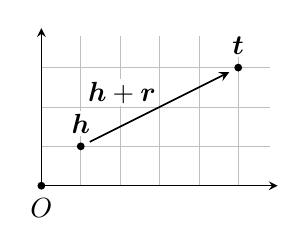
\begin{tikzpicture}
  \draw [lightgray, very thin, step = 0.5] (0, 0) grid (2.9, 1.9);
  \draw [arrow, <->, thin, shorten > = 0pt, shorten < = 0pt] (0, 2) -- (0, 0) -- (3, 0);
  \node [circle, fill, inner sep = 1pt, label = below:$O$] at (0, 0) {};
  \node (h) [circle, fill, inner sep = 1pt, label = $\bm{h}$] at (0.5, 0.5) {};
  \node (t) [circle, fill, inner sep = 1pt, label = $\bm{t}$] at (2.5, 1.5) {};
  \draw [arrow] (h) -- node [midway, auto, fill = white, inner sep = 1pt] {$\bm{h} + \bm{r}$} (t);
\end{tikzpicture}

  \caption{%
    The TransE model\cite{Bordes2013} aims to satisfy $\bm{h} + \bm{r} = \bm{t}$ for every triple $(h, r, t)$.
    In this case $\bm{h} = (0.5, 0.5)$, $\bm{t} = (2.5, 1.5)$, and $\bm{r} = (2, 1)$.%
  }\label{fig:transe}
\end{figure}

It should be noted that the embedding in \figurename~\ref{fig:transe} inhibits the $\mathbb{R}^2$ space since it makes for an intuitive illustration.
However, a graph embedding usually occupies a space of higher dimensions since it allows for more details to be captured.

It is clear that if a TransE embedding satisfies $\bm{h} + \bm{r} = \bm{t}$, we can use $\bm{h} + \bm{r} - \bm{t}$ as a measure of correctness; the closer the value of $f$ is to $0$, the more correct the embedding is.
This leads to the TransE score function which is defined as $f(h, r, t) = - \Vert \bm{h} + \bm{r} - \bm{t} \Vert_p^2$.
Here, $\Vert\cdot\Vert_p$ denotes the $p$-norm which has the general form
\[\Vert \bm{e} \Vert_p = \sqrt[p]{\bm{e}_1^p + \bm{e}_2^p + \cdots + \bm{e}_i^p}.\]
If the TransE embedding is perfect, true triples will have a score of $0$ while false triples will have negative scores.

TransE is a simple model but it lacks the ability to model complicated relations often found in \acp{kg}.
Examples of these are
\begin{enumerate*}
  \item symmetric relations where both $(h, r, t)$ and $(t, r, h)$ are present,
  \item inverse relations where $r$ is an inverse of $r'$ if both $(h, r, t)$ and $(t, r', h)$ exist, and
  \item composed relations where $r$ is a composition of $r'$ and $r''$ if $(h, r, t)$, $(h, r', t')$, and $(t', r'', t)$ are present.
\end{enumerate*}
This is an issue addressed by the RotatE approach\cite{Sun2019}.
This technique embeds triples into a complex embedding space where relations represent rotational translations between entities.
More specifically, given a triple $(h, r, t)$, RotatE aims to satisfy $\bm{h} \circ \bm{r} = \bm{t}$.
Here, $\circ$ denotes the element-wise product of two vectors, meaning that if $\bm{t} = \bm{h} \circ \bm{r}$ then ${\bm{t}}_i = {\bm{h}}_i \bm{r}_i$.
The advantage of RotatE is that it is capable of modelling the different types of relations described above.

In addition to complicated relations, \acp{kg} often also exhibit semantic hierarchies.
For instance, in the medical domain, drugs are grouped in different categories such as antipyretics and vaccines.
The \ac{hake} technique\cite{Zhang2019}, which build upon RotatE, is developed specifically to handle such structures.
The purpose of the technique is to persist semantic hierarchies in the graph embedding.
This is done by dividing the embedding of entities into two parts: one that represents their hierarchical levels and one that distinguishes them on the same level.
Then the relation embeddings act as translations between the entities.

A \ac{kg} embedding can be used for link prediction by passing candidate triples through the score function.
The triples that get assigned the highest scores are most likely to exist.
The \ac{hake} technique currently produces state-of-the-art results for this link prediction task, which is why we take a closer look at it in the next section.


\section{The \ac{hake} Technique}\label{sec:method}

This section will cover the intuition behind the \ac{hake} technique and how it is used for link prediction.
We start, in Section~\ref{sec:representing-hieraricies}, by giving an intuitive understanding of the technique by introducing its overall goal and concrete concepts.
In Section~\ref{sec:learning}, we take a look at how these concepts are deployed in a learning setting.

\subsection{Representing Hierarchies in Embeddings}\label{sec:representing-hieraricies}

As stated earlier, the \ac{hake} technique embeds entities and relations into a polar coordinate system.
In such coordinate system, a point is described by its distance from the origin as well as its angle relative to a reference direction.
These constituents are referred to as the radial coordinate, denoted $\rho$, and angular coordinate, denoted $\phi$, respectively.
Given an embedded entity $\bm{e} = (\bm{e}_\rho, \bm{e}_\phi)$, we use $\bm{e}_\rho$ to denote the radial part and $\bm{e}_\phi$ to denote the angular part of the corresponding entity.
This is illustrated in \figurename~\ref{fig:polar} where the entity $\bm{e}$ has radial coordinate $2$ and angular coordinate $0.8$.
As in TransE, embeddings usually live in a high dimensional space.
For the sake of illustrative examples, however, we use the $\mathbb{R}^2$ space.

\begin{figure}[ht]
  \centering\small
  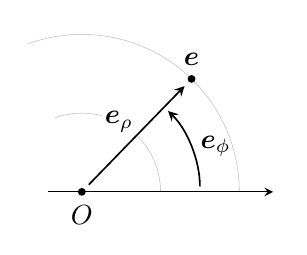
\begin{tikzpicture}
  \node (o) [circle, fill, inner sep = 1pt, label = below:$O$] at (0, 0) {};
  \draw [draw, lightgray, very thin] (1, 0) arc (0:110:1);
  \draw [draw, lightgray, very thin] (2, 0) arc (0:110:2);
  \draw [arrow, thin] (-0.5, 0) -- (2.5, 0);
  \node (e) [circle, fill, inner sep = 1pt, label = $\bm{e}$] at (0.8r:2cm) {};
  \draw [arrow] (o) -- node [midway, auto, fill = white, inner sep = 1pt] {$\bm{e}_\rho$} (e);
  \draw [arrow] (1.5, 0) arc (0:0.8r:1.5) node [midway, right] {$\bm{e}_\phi$};
\end{tikzpicture}

  \caption{The embedded entity $\bm{e} = (2, 0.8)$ in the polar coordinate system.}\label{fig:polar}
\end{figure}

The motivation behind this two-fold embedding is, as mentioned earlier, that each component models a distinct aspect of the entity.
\figurename~\ref{fig:hierarchy} illustrates entities from a medical domain.
Here, \textsc{drug} is the most general entity and thus lies at the top of the hierarchy.
One step down the hierarchy and we get a certain class of drugs, \textsc{antipyretics}.
The entities \textsc{aspirin} and \textsc{ibuprofen} are instances of \textsc{antipyretics} and thus represent another step down the hierarchy.
Entities on the same level of the hierarchy have the same radial coordinate and different angular coordinates.

\begin{figure}[ht]
  \centering\small
  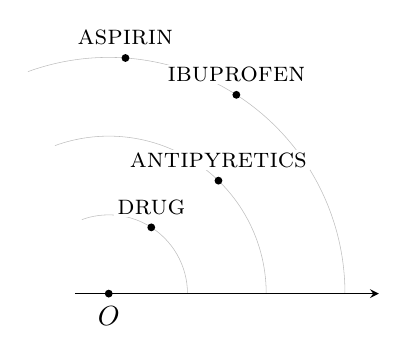
\begin{tikzpicture}
  \node [circle, fill, inner sep = 1pt, label = below:$O$] at (0, 0) {};
  \draw [draw, lightgray, very thin] (1, 0) arc (0:110:1);
  \draw [draw, lightgray, very thin] (2, 0) arc (0:110:2);
  \draw [draw, lightgray, very thin] (3, 0) arc (0:110:3);
  \draw [arrow, thin] (-0.5, 0) -- (3.5, 0);

  \node [circle, fill, inner sep = 1pt, label = \textsc{drug}] at (1r:1cm) {};
  \node [circle, fill, inner sep = 1pt, label = \textsc{antipyretics}] at (0.8r:2cm) {};
  \node [circle, fill, inner sep = 1pt, label = \textsc{aspirin}] at (1.5r:3cm) {};
  \node [circle, fill, inner sep = 1pt, label = \textsc{ibuprofen}] at (1r:3cm) {};
\end{tikzpicture}

  \caption{The goal of the representation in the \ac{hake} technique is that entities of the same hierarchical level, such as \textsc{aspirin} and \textsc{ibuprofen}, have similar radial coordinates but different angular coordinates.}\label{fig:hierarchy}
\end{figure}

Since the \ac{hake} technique relies on a translational model like TransE and RotatE, it aims to achieve a similar goal.
For each triple $(h, r, t)$, the embedded relation $\bm{r}$ acts as a translation from $\bm{h}$ to $\bm{t}$.
Since each entity consists of two parts, radial and angular, the objective of this translation is two-fold.
For the radial coordinate, the translation is a scaling operation, i.e.\ for each triple $(h, r, t)$, we want to satisfy
\begin{equation}\label{eq:radial-translation}
  \bm{h}_\rho \circ \bm{r}_\rho = \bm{t}_\rho.
\end{equation}
Once again, the $\circ$ operator is the element-wise product, i.e.\ ${\bm{h}_\rho}_i{\bm{r}_\rho}_i = {\bm{t}_\rho}_i$.
This is what allows the translation to move from one level of the semantic hierarchy, namely $\bm{h}_\rho$, to another level $\bm{t}_\rho$.

For the angular coordinate, the translation is a rotation that, for each triple $(h, r, t)$, should satisfy
\begin{equation}\label{eq:angular-translation}
  \bm{h}_\phi + \bm{r}_\phi \bmod{2\pi} = \bm{t}_\phi.
\end{equation}
The angular translation of an entity $\bm{e} = (\bm{e}_\rho, \bm{e}_\phi)$ can be seen as moving along the circumference of a circle with radius $\bm{e}_\rho$ starting at angle $\bm{e}_\phi$ \si{\radian}.
This translation has a periodic nature in the interval $[0;2\pi]$ which is the reason for the modulo operator in (\ref{eq:angular-translation}).

\begin{example}[Relations as translations]\label{ex:translation}
  To illustrate how a relation acts as a translation from one entity to another, we consider \figurename~\ref{fig:translation} that shows an embedding of the triple $(h, r, t)$.
  Here, we assume $\bm{h} = (1, 0.3)$, $\bm{t} = (3, 0.8)$, and $\bm{r} = (3, 0.5)$.
  This embedding satisfies (\ref{eq:radial-translation}) and (\ref{eq:angular-translation}) since $1 \cdot 3 = 3$ and $0.3 + 0.5 \bmod 2\pi = 0.8$ respectively.

  \begin{figure}[ht]
    \centering\small
    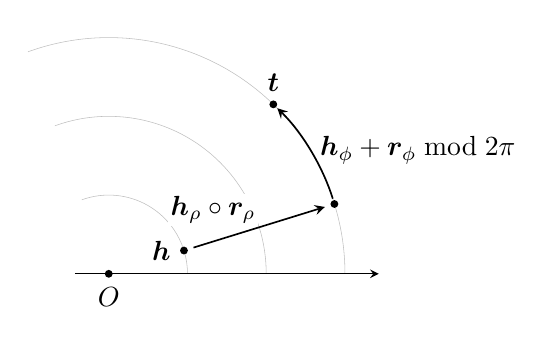
\begin{tikzpicture}
  \node [circle, fill, inner sep = 1pt, label = below:$O$] at (0, 0) {};
  \draw [draw, lightgray, very thin] (1, 0) arc (0:110:1);
  \draw [draw, lightgray, very thin] (2, 0) arc (0:110:2);
  \draw [draw, lightgray, very thin] (3, 0) arc (0:110:3);
  \draw [arrow, thin] (-0.5, 0) -- (3.5, 0);

  \node (h) [circle, fill, inner sep = 1pt, label = left:$\bm{h}$] at (0.3r:1cm) {};
  \node (t) [circle, fill, inner sep = 1pt, label = above:$\bm{t}$] at (0.8r:3cm) {};
  \node (hm) [circle, fill, inner sep = 1pt] at (0.3r:3cm) {};

  \draw [arrow] (h) -- node [midway, auto, inner sep = 1pt, fill = white] {$\bm{h}_\rho \circ \bm{r}_\rho$} (hm);
  \draw [arrow] ([shift=(0.3r:3cm)]0, 0) arc (0.3r:0.8r:3cm) node [midway, right] {$\bm{h}_\phi + \bm{r}_\phi \bmod 2\pi$};
\end{tikzpicture}

    \caption{When the triple $(h, r, t)$ is embedded, the relation $\bm{r} = (3, 0.5)$ acts as a translation from $\bm{h} = (1, 0.3)$ to $\bm{t} = (3, 0.8)$.}\label{fig:translation}
  \end{figure}
\end{example}

When learning the embedding, we must define a measure of similarity or dissimilarity between our current embedding of a triple $(h, r, t)$, and a true perfect embedding.
We do this through a distance function which intuitively describes how good an embedding is at satisfying (\ref{eq:radial-translation}) and (\ref{eq:angular-translation}).
For the radial and angular component, we define separate distance functions.
For the radial component, we have the distance function
\begin{equation}\label{eq:distance-function-radial}
  \text{d}_\rho(\bm{h}, \bm{r}, \bm{t}) = \Vert \bm{h}_\rho \circ \bm{r}_\rho - \bm{t}_\rho \Vert_2
\end{equation}
and for the angular component, the distance function is defined as
\begin{equation}\label{eq:distance-function-angular}
  \text{d}_\phi(\bm{h}, \bm{r}, \bm{t}) = \left\Vert \sin \frac{\bm{h}_\phi + \bm{r}_\phi - \bm{t}_\phi}{2} \right\Vert_1.
\end{equation}
We define the final distance function as the sum of (\ref{eq:distance-function-radial}) and (\ref{eq:distance-function-angular}) as seen in (\ref{eq:distance-function}).
\begin{equation}\label{eq:distance-function}
  \text{d}(\bm{h}, \bm{r}, \bm{t}) = \text{d}_\rho(\bm{h}, \bm{r}, \bm{t}) + \text{d}_\phi(\bm{h}, \bm{r}, \bm{t})
\end{equation}
It is clear that if the embedding is perfect, we will have $\text{d}(\bm{h}, \bm{r}, \bm{t}) = 0$ for every triple $(h, r, t)$.
Similarly, the more off the embedding is, the larger the distance value.

\begin{example}[Distance functions]
  We reconsider \figurename~\ref{fig:translation} from Example~\ref{ex:translation}.
  Applying (\ref{eq:distance-function}) to the valid triple $(h, r, t)$ gives us a distance of
  \[\sqrt{{(1 \cdot 3 - 3)}^2} + \sin \frac{0.3 + 0.5 - 0.8}{2} = 0\]
  as expected.
  Now, assume we introduce a new triple $(h, r', t)$ to the \ac{kg}.
  Initially, we have $\bm{r'} = (2, 1.3)$ and by applying the distance function (\ref{eq:distance-function}) we get
  \[\sqrt{{(1 \cdot 2 - 3)}^2} + \sin \frac{0.3 + 1.3 - 0.8}{2} = 1.389.\]
  This will get penalised in the learning process and the embedding of $r'$ will be adjusted.
\end{example}

\subsection{Learning the Embedding}\label{sec:learning}

For the learning process, we must first define the score function.
In the \ac{hake} technique, the distance function (\ref{eq:distance-function}) is at the core of the score function.
However, to satisfy the property that the score function must assign high scores to correct embeddings and lower scores to wrong embeddings, we invert the sign as seen in (\ref{eq:score-function}).
In this way, a perfect embedding will get the highest score $0$.
\begin{equation}\label{eq:score-function}
  f(\bm{h}, \bm{r}, \bm{t}) = - \text{d}(\bm{h}, \bm{r}, \bm{t})
\end{equation}

Furthermore, the weights $\lambda$ and $\mu$ are added to each term in the distance function.
These weights are treated as hyperparameters and will be learned by the model together with the entity and relation embeddings.
\begin{equation}
  \text{d}(\bm{h}, \bm{r}, \bm{t}) = \lambda\text{d}_\rho(\bm{h}, \bm{r}, \bm{t}) + \mu\text{d}_\phi(\bm{h}, \bm{r}, \bm{t})
\end{equation}

The \ac{hake} method uses negative sampling\cite{Mikolov2013} when learning the embedding.
The purpose of this sampling technique is to cope with the softmax function typically used when learning classification problems.
The softmax function maps a real-valued vector to a vector of numbers between 0 and 1 that can be treated as a probability distribution.
Given a \ac{kg} $\mathcal{K}$ and a score function $f$, we can compute the softmax value for a triple $(h, r, t) \in \mathcal{K}$ as

\[\frac{e^{f(\bm{h}, \bm{r}, \bm{t})}}{\sum_{(h', r', t') \in \mathcal{K}} e^{f({\bm{h'}, \bm{r'}, \bm{t'}})}}.\]

The problem here is the summation in the denominator which becomes increasingly expensive to compute as the \ac{kg} grows.
According to\cite{Paulheim2016}, many freely available \acp{kg} contain billions of facts making softmax computation infeasible.

Negative sampling provides a way around this by generating a number of negative triples $(h', r, t') \not\in \mathcal{K}$ for every positive triple $(h, r, t) \in \mathcal{K}$.
Based on a positive triple $(h, r, t)$, a negative triple is either on the form $(h', r, t)$ or $(h, r, t')$ where $h'$ and $t'$ are sampled from the entities in the \ac{kg}.
For convenience, we describe negative triples given a positive triple $(h, r, t)$ as the set
\begin{equation}\label{eq:negative-samples}
  \begin{split}
    \mathcal{N}_{(h, r, t)} = {} & \{(h, r, t') \mid t' \in \mathcal{E} \wedge (h, r, t') \not\in \mathcal{K}\} \\
    & \cup \{(h', r, t) \mid h' \in \mathcal{E} \wedge (h', r, t) \not\in \mathcal{K}\}.
  \end{split}
\end{equation}
Furthermore, we use the notation $\mathcal{N}_{{(h, r, t)}_n}$ for the set of $n$ uniformly sampled negative triples.

As in many other machine learning problems, we wish to minimise a certain loss function in the learning process.
We use the distance function (\ref{eq:distance-function}) and negative sampling to define the loss function as
\begin{equation}\label{eq:loss-function}
  \begin{split}
    & - \log\sigma(\gamma - \text{d}(\bm{h}, \bm{r}, \bm{t})) \\
    &- \sum_{\mathclap{(h', r, t') \in \mathcal{N}_{{(h, r, t)}_n}}} P(h', r, t')\log\sigma(\text{d}(\bm{h'}, \bm{r}, \bm{t'}) - \gamma),
  \end{split}
\end{equation}
where $\gamma$ is a positive margin parameter and $\sigma$ is the sigmoid function,
\[\sigma(x) = \frac{1}{1 + e^{-x}}.\]

To get an intuition of (\ref{eq:loss-function}), we notice two things.
First, from (\ref{eq:distance-function}) we know that the value of the distance function cannot be negative.
Second, we note that the value of $\log\sigma(\cdot)$ grows as its parameter increases.
Therefore, the first term gets the lowest value when $\text{d}(\bm{h}, \bm{r}, \bm{t}) = 0$.
In the second term, the order of $\gamma$ and $\text{d}(\bm{h}, \bm{r}, \bm{t})$ is flipped.
This means that the value for the second term gets lower as the distances of the negative triples get higher.
Immediately, this satisfies the objectives of the \ac{hake} discussed in the previous section.
Moreover, each negative triple in (\ref{eq:loss-function}) is multiplied by a weight $P$ defined as
\[P(h', r, t') = \frac{e^{\alpha f(\bm{h'}, \bm{r}, \bm{t'})}}{\sum_{(h'', r, t'') \in \mathcal{N}_{{(h, r, t)}_n}} e^{\alpha f(\bm{h''}, \bm{r}, \bm{t''})}},\]
where $\alpha$ is the sampling temperature.

Contrary to what we described earlier, this weight is actually a softmax distribution.
In this case, the computation is not problematic since it is dependent on a fixed size of samples, namely the negative sample size $n$, and not the size of the entire dataset $|\mathcal{K}|$.

Now, with all necessary concepts defined, we formulate the learning process which is illustrated in \figurename~\ref{alg:learning}.
First, we initialise the entity and relation embeddings on Line~\ref{alg:learning:ent} and~\ref{alg:learning:rel}.
This is done by creating an embedding vector $\bm{e} \in \mathbb{R}^{d2}$ for each $e \in \mathcal{E}$ and setting its entries $\bm{e}_i$ to values drawn from the uniform distribution $\mathcal{U}$.
The relation embeddings go through the same procedure.
The main learning loop is based on mini-batch gradient decent using the Adam optimiser\cite{Kingma2014}.
In each iteration, we sample a batch of $b$ true triples $\mathcal{B}^+$ from the training dataset $\mathcal{K}$ on Line~\ref{alg:learning:pos-batch}.
For each true triple, we sample $n$ negative triples in the batch $\mathcal{B}^-$ on Line~\ref{alg:learning:neg-batch}.
Together, these form the training batch $\mathcal{B}$ composed of pairs of a true triple and a set of negative triples as seen on Line~\ref{alg:learning:batch}.
Based on $\mathcal{B}$, we compute the sum of losses using (\ref{eq:loss-function}) and update the parameters of the model by taking a gradient step on Line~\ref{alg:learning:loss}.
The parameters that get updated are the entity embedding, the relation embedding, the radial weight $\lambda$, and the angular weight $\mu$.

\begin{figure*}
  \caption{Pseudo code for the training procedure of the \ac{hake} technique inspired by\cite{Bordes2013}.}\label{alg:learning}
  \begin{algorithmic}[1]
    \Require Training dataset $\mathcal{K} = \{(h, r, t) \mid h, t \in \mathcal{E} \wedge r \in \mathcal{R}\}$, dimensionality of embedding space $d$, margin $\gamma$, batch size $b$, and negative sample size $n$.
    \Statex
    \State $\bm{e}_i \gets \mathcal{U}(-\frac{\gamma}{d}, \frac{\gamma}{d})$ for each $e \in \mathcal{E}$, where $\bm{e} \in \mathbb{R}^{2d}$ \label{alg:learning:ent}
    \State $\bm{r}_i \gets \mathcal{U}(-\frac{\gamma}{d}, \frac{\gamma}{d})$ for each $r \in \mathcal{R}$, where $\bm{r} \in \mathbb{R}^{2d}$ \label{alg:learning:rel}
    \Loop
    \State $\mathcal{B} \gets \emptyset$
    \State $\mathcal{B}^+ \gets \text{sample}(\mathcal{K}, b)$ \label{alg:learning:pos-batch}
    \For{$(h, r, t) \in \mathcal{B}^+$}
    \State $\mathcal{B}^- \gets \text{sample}(\mathcal{N}_{(h, r, t)}, n)$ \label{alg:learning:neg-batch}
    \State $\mathcal{B} \gets \mathcal{B} \cup \{\big((h, r, t), \mathcal{B}^-\big)\}$ \label{alg:learning:batch}
    \EndFor
    \State Update parameters w.r.t $\displaystyle\sum_{\mathclap{((h, r, t), \mathcal{B}^-) \in \mathcal{B}}} \nabla \big(- \log\sigma(\gamma - \text{d}(\bm{h}, \bm{r}, \bm{t})) - \sum_{\mathclap{(h', r, t') \in \mathcal{B}^-}} P(h', r, t') \log\sigma(\text{d}(\bm{h'}, \bm{r}, \bm{t'}) - \gamma)\big)$ \label{alg:learning:loss}

    \EndLoop
  \end{algorithmic}
\end{figure*}


\section{Experiments}\label{sec:experiments}

We conduct two different experiments in the following sections to evaluate the \ac{hake} technique for link prediction.
While both use the same setup and evaluation methods, they examine different aspects of the technique.
In Section~\ref{sec:setup}, we cover the setup of both experiments as well as the metrics used for evaluation.
Section~\ref{sec:replication} and~\ref{sec:domain-specific} explain the different experiments and present their results.

\subsection{Setup and Evaluation Metrics}\label{sec:setup}

The testing procedure used for the \ac{hake} technique originate from TransE\cite{Bordes2013} and has been used to evaluate a variety of related link prediction methods.
The core of the test dataset is a set of true triples $\mathcal{S}$ that do not overlap with the training data $\mathcal{K}$.
For each true triple $(h, r, t) \in \mathcal{S}$, we generate a set of false triples by replacing either $h$ or $t$ by entities sampled from the \ac{kg}.
The union of the true and false triples make up the final test dataset $\mathcal{S'}$.
It should be noted that following this generating process may produce triples that appear in the training or validation datasets.
Therefore, to avoid skewed results, we remove such triples from the test dataset.
Generally, given a set of true test triples $\mathcal{S}$ over entities $\mathcal{E}$ and a set training triples $\mathcal{K}$, we can formulate the test dataset as

\begin{equation*}
  \begin{split}
    \mathcal{S'} = {} & \mathcal{S} \cup \{(h, r, t') \mid (h, r, t) \in \mathcal{S} \wedge t' \in \mathcal{E} \wedge (h, r, t') \not\in \mathcal{K}\} \\
    & \cup \{(h', r, t) \mid (h, r, t) \in \mathcal{S} \wedge h' \in \mathcal{E} \wedge (h', r, t) \not\in \mathcal{K}\}.
  \end{split}
\end{equation*}

The triples in $\mathcal{S'}$ are now ranked by their score (\ref{eq:score-function}) such that the triple with the highest score is assigned rank $1$ and the triple with the lowest score is assigned rank $|\mathcal{S'}|$.

For evaluation, we use the measures \ac{mrr} and \ac{han} since they are widely adopted for link prediction techniques.
The \ac{mrr} is calculated as
\begin{equation}\label{eq:mrr}
  \text{\ac{mrr}} = \frac{1}{|\mathcal{S}|} \sum_{(h, r, t) \in \mathcal{S}} \frac{1}{\text{rank}(h, r, t)}.
\end{equation}

Here, $\mathcal{S}$ is the set of true triples and the rank function returns the rank of a triple in entire test dataset $\mathcal{S'}$.
Clearly, as more true triples are assigned low ranks, meaning that their reciprocal ranks are high, the \ac{mrr} increases.
Also worth noticing is that as we move down the ranked list of triples, the exact rank of a true triple has less impact on the overall \ac{mrr}.
That is, a change in rank from $200$ to $199$ has minimal impact compared to a change from $2$ to $1$.

The \ac{han} measure is also based on the ranked set of triples.
Given an $n$, the \ac{han} value is the proportion of correct predictions in the first $n$ elements of the ranked list as seen below.
\begin{equation}\label{eq:han}
  \text{\ac{han}} = \frac{|\text{correct predictions}|}{n}
\end{equation}

Similarly \ac{mrr}, a higher \ac{han} value is better.
If all of the top $n$ ranked triples are true, the \ac{han} will be $1$.

For the sake of replication, we run both experiments using the Python implementation of the \ac{hake} technique from\cite{Zhang2019}.\footnote{The code for the original \ac{hake} paper is available on Github: \url{https://github.com/MIRALab-USTC/KGE-HAKE}.}
This implementation is based on the neural network library PyTorch.

\subsection{Replication}\label{sec:replication}

This experiment is carried out by running the exact experiments presented in\cite{Zhang2019}.
Here, the \ac{hake} technique is evaluated on the three standard datasets WN18RR, FB15k-237, and YAGO3\--10 that are based on the \acp{kg} WordNet, Freebase, and \ac{yago} respectively.
In the original experiments, the authors perform hyperparameter optimisation to find the best parameter configurations for each dataset.
We use the same parameter configurations in the replication experiments.

The results of the replication experiments are shown in Table~\ref{tab:replication}.
The bottom row indicates how many percent the replicated results deviate from the original results.
This deviation is calculated by
\[\frac{\text{replication} - \text{original}}{\text{replication}} \cdot \SI{100}{\percent}.\]

\begin{table*}[ht]
  \centering
  \caption{Results for Replication Experiment}\label{tab:replication}
  \subsection{Replication}\label{sec:replication}

This experiment is carried out by running the exact experiments presented in\cite{Zhang2019}.
Here, the \ac{hake} technique is evaluated on the three standard datasets WN18RR, FB15k-237, and YAGO3\--10 that are based on the \acp{kg} WordNet, Freebase, and \ac{yago} respectively.
In the original experiments, the authors perform hyperparameter optimisation to find the best parameter configurations for each dataset.
We use the same parameter configurations in the replication experiments.

The results of the replication experiments are shown in Table~\ref{tab:replication}.
The bottom row indicates how many percent the replicated results deviate from the original results.
This deviation is calculated by
\[\frac{\text{replication} - \text{original}}{\text{replication}} \cdot \SI{100}{\percent}.\]

\begin{table*}[ht]
  \centering
  \caption{Results for Replication Experiment}\label{tab:replication}
  \input{sections/experiments/tables/replication.tex}
\end{table*}

By looking at the deviation, it is clear that the different datasets give rise to different results.
On the WordNet dataset, the replication experiment ranges from performing \SI{-1.77}{\percent} worse to \SI{0.172}{\percent} better.
We do not consider this a significant deviation and it could just be due to differences in the initialisation of the entity and relation embeddings.
However, replication results on the Freebase and \ac{yago} datasets are much different from the original results.
Worth noticing is that the replication results are consistently worse than the original.
This indicates that the difference in performance is not only due to differences in the initial embeddings as suggested for the WordNet dataset.
It should be noted, however, that due to limitations on computational power, we have not been able to run the experiments more than a few times per dataset.
This is in contrast to the results in\cite{Zhang2019} which are averages of multiple runs.
Nonetheless, we think that a \SIrange{-3.58}{-11.7}{\percent} deviation is significant.

\end{table*}

By looking at the deviation, it is clear that the different datasets give rise to different results.
On the WordNet dataset, the replication experiment ranges from performing \SI{-1.77}{\percent} worse to \SI{0.172}{\percent} better.
We do not consider this a significant deviation and it could just be due to differences in the initialisation of the entity and relation embeddings.
However, replication results on the Freebase and \ac{yago} datasets are much different from the original results.
Worth noticing is that the replication results are consistently worse than the original.
This indicates that the difference in performance is not only due to differences in the initial embeddings as suggested for the WordNet dataset.
It should be noted, however, that due to limitations on computational power, we have not been able to run the experiments more than a few times per dataset.
This is in contrast to the results in\cite{Zhang2019} which are averages of multiple runs.
Nonetheless, we think that a \SIrange{-3.58}{-11.7}{\percent} deviation is significant.

\subsection{Domain-Specific Data}\label{sec:domain-specific}

The goal of this experiment is to find out how the \ac{hake} technique performs on domain-specific data which, compared to the data used in the replication experiment, is non-standard.
We construct a \ac{kg} specific for the medical domain by extracting data from Wikidata using its SPARQL endpoint.\footnote{The code used for dataset construction can be found on Github: \url{https://github.com/emilbaekdahl/p8-code}. It is also attached to the hand-in of this project.}
In the construction, we explicitly include a class-subclass-instance hierarchy.
In Wikidata, the hierarchy is based on the relations \textsc{subclass of}\footnote{\url{https://www.wikidata.org/wiki/Property:P279}} and \textsc{instance of}\footnote{\url{https://www.wikidata.org/wiki/Property:P31}}.
As an example, we consider the entity \textsc{medication}\footnote{\url{https://www.wikidata.org/wiki/Q12140}}, one of the most general entities in the \ac{kg}, that occurs in the triple $(\textsc{antipyretic}, \textsc{subclass of}, \textsc{medication})$ which in turn occurs in $(\textsc{aspirin}, \textsc{instance of}, \textsc{antipyretic})$.

We believe that this way of constructing the \ac{kg} with a clear hierarchy makes it suitable for the \ac{hake} technique.
However, it should be noted that\cite{Zhang2019} does not mention any requirements to the hierarchy; for instance, if it must be balanced or strict.
This means that, in the domain-specific \ac{kg}, an entity can be related to entities at different levels of the hierarchy.
An example of this seen in \figurename~\ref{fig:non-strict-hierarchy} where \textsc{aspirin} is both an instance of \textsc{antipyretic} and \textsc{medication} even though those entities occupy two different levels of the hierarchy.

\begin{figure}[ht]
  \centering\small
  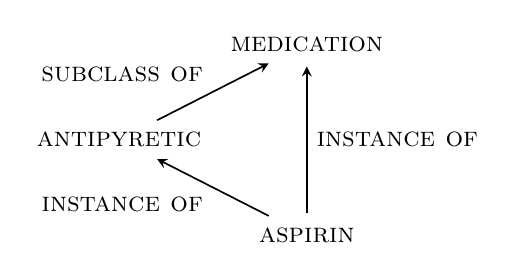
\begin{tikzpicture}[font = \scshape]
  \node (med) {medication};
  \node (anti) [below left = 1cm and 0.125cm of med, anchor = east] {antipyretic};
  \node (asp) [below = 2cm of med] {aspirin};

  \draw [arrow] (anti) -- node [auto] {subclass of} (med);
  \draw [arrow] (asp) -- node [auto] {instance of} (anti);
  \draw [arrow] (asp) -- node [auto, right] {instance of} (med);
\end{tikzpicture}

  \caption{%
    The \ac{hake} technique does not require a specific structure to the hierarchies in the \ac{kg}.
    This means that we, for instance, find non-strict hierarchies in the domain-specific \ac{kg}, where an entity is related to multiple entities at different hierarchical levels.
  }\label{fig:non-strict-hierarchy}
\end{figure}

The medical dataset has \num{20422} entities, \num{5} types of relations, and a total of \num{34216} facts.
The results from the experiment with domain-specific data is shown in Table~\ref{tab:domain-specific} where the replication experiment results from Table~\ref{tab:replication} is included for comparison.
We clearly see a significant decrease in performance on the domain-specific dataset.

\begin{table}[ht]
  \centering
  \caption{Results for Domain-Specific Dataset Experiment}\label{tab:domain-specific}
  \subsection{Domain-Specific Data}\label{sec:domain-specific}

The goal of this experiment is to find out how the \ac{hake} technique performs on domain-specific data which, compared to the data used in the replication experiment, is non-standard.
We construct a \ac{kg} specific for the medical domain by extracting data from Wikidata using its SPARQL endpoint.\footnote{The code used for dataset construction can be found on Github: \url{https://github.com/emilbaekdahl/p8-code}. It is also attached to the hand-in of this project.}
In the construction, we explicitly include a class-subclass-instance hierarchy.
In Wikidata, the hierarchy is based on the relations \textsc{subclass of}\footnote{\url{https://www.wikidata.org/wiki/Property:P279}} and \textsc{instance of}\footnote{\url{https://www.wikidata.org/wiki/Property:P31}}.
As an example, we consider the entity \textsc{medication}\footnote{\url{https://www.wikidata.org/wiki/Q12140}}, one of the most general entities in the \ac{kg}, that occurs in the triple $(\textsc{antipyretic}, \textsc{subclass of}, \textsc{medication})$ which in turn occurs in $(\textsc{aspirin}, \textsc{instance of}, \textsc{antipyretic})$.

We believe that this way of constructing the \ac{kg} with a clear hierarchy makes it suitable for the \ac{hake} technique.
However, it should be noted that\cite{Zhang2019} does not mention any requirements to the hierarchy; for instance, if it must be balanced or strict.
This means that, in the domain-specific \ac{kg}, an entity can be related to entities at different levels of the hierarchy.
An example of this seen in \figurename~\ref{fig:non-strict-hierarchy} where \textsc{aspirin} is both an instance of \textsc{antipyretic} and \textsc{medication} even though those entities occupy two different levels of the hierarchy.

\begin{figure}[ht]
  \centering\small
  \input{sections/experiments/figures/non-strict-hierarchy.tex}
  \caption{%
    The \ac{hake} technique does not require a specific structure to the hierarchies in the \ac{kg}.
    This means that we, for instance, find non-strict hierarchies in the domain-specific \ac{kg}, where an entity is related to multiple entities at different hierarchical levels.
  }\label{fig:non-strict-hierarchy}
\end{figure}

The medical dataset has \num{20422} entities, \num{5} types of relations, and a total of \num{34216} facts.
The results from the experiment with domain-specific data is shown in Table~\ref{tab:domain-specific} where the replication experiment results from Table~\ref{tab:replication} is included for comparison.
We clearly see a significant decrease in performance on the domain-specific dataset.

\begin{table}[ht]
  \centering
  \caption{Results for Domain-Specific Dataset Experiment}\label{tab:domain-specific}
  \input{sections/experiments/tables/domain-specific.tex}
\end{table}

\end{table}


\section{Discussion}\label{sec:discussion}

From the experiments in the previous section, we found problems with result replication of the \ac{hake} paper and that the technique does not perform well on domain-specific data.
In this section, we provide possible explanations for those encountered problems, and discuss how future research may address the link prediction problem differently.

\subsection{Evaluation Protocol}

Most link prediction methods that stem from the TransE model\cite{Bordes2013}, such as the \ac{hake} technique, are evaluated on the same standard datasets that we introduced in Section~\ref{sec:replication}.
Immediately, this gives a good foundation for comparing the different techniques.
However, if those datasets are not realistic, the measures do not say much about how the techniques perform in real-world applications.
Therefore, it is worth looking at the structure and content of WordNet, Freebase, \ac{yago}, and alike.
This issue is addressed in\cite{Akrami2020}.
It turns out that the standard datasets WN18RR, FB15k-237, and YAGO3\--10 suffer from two major problems: data redundancy and Cartesian product relations.

Data redundancy is primarily caused by many pairs of triples being reverse of each other, that is both $(h, r, t)$ and $(t, r^{-1}, h)$ being present in the data.
Here $r^{-1}$ symbolises the reverse of the relation $r$.
An example of this can be found in Wikidata where the relations \textsc{medical condition treated}\footnote{\url{https://www.wikidata.org/wiki/Property:P2175}} and \textsc{drug used for treatment}\footnote{\url{https://www.wikidata.org/wiki/Property:P2176}} can give rise to the triple $(\textsc{aspirin}, \textsc{medical condition treated}, \textsc{pain})$ which is a reverse of $(\textsc{pain}, \textsc{drug used for treatment}, \textsc{aspirin})$.
In~\cite{Akrami2020}, the authors find that, in datasets with many reverse triple pairs, a simple rule-based link prediction method performs on par with, or sometimes even better than, graph embedding-based techniques.
Such rules for predicting reverse triples can be derived from statistical measures of the dataset\cite{Dettmers2017}.
Given two relations $r$ and $r'$, we compute the proportion of triples $(h, r, t)$ where $h$ and $t$ are reversely related by $r'$, that is $(t, r', h)$.
This measure can be described as
\[\frac{|\{(h, r, t) \mid (h, r, t) \in \mathcal{K} \wedge (t, r', h) \in \mathcal{K}\}|}{|\{(h, r, t) \mid (h, r, t) \in \mathcal{K}\}|}.\]
If this proportion exceeds a given threshold, say $0.8$, we conclude the rule
\[(h, r, t) \implies (t, r', h).\]
Repeating this for each pair of relations $(r, r') \in \mathcal{R} \times \mathcal{R}$ will produce a rule-based classifier that yields an H@1 value around $0.7$ on certain datasets\cite{Akrami2020}.

Cartesian product relations occur when all elements in a set of head entities $H$ are connected to all elements in a set of tail entities $T$ with a given relation $r$, that is $\{(h, r, t) \mid (h, r, t) \in \mathcal{K} \wedge (h, t) \in H \times T\}$.
The primary issue with Cartesian product relations is that they typically give rise to unrealistic link prediction tasks.
According to\cite{Akrami2020}, these types of relations often occur when mediator nodes are used to simplify complicated relations between entities.
For instance, if we wanted to extend the \ac{kg} in \figurename~\ref{fig:one-fact-kb-graph} such that the treatment of pain with aspirin is related to the side-effect nausea, we use a mediator node \textsc{treatment}.
An illustration of this can be seed in \figurename~\ref{fig:mediator}.

\begin{figure}[ht]
  \small\centering
  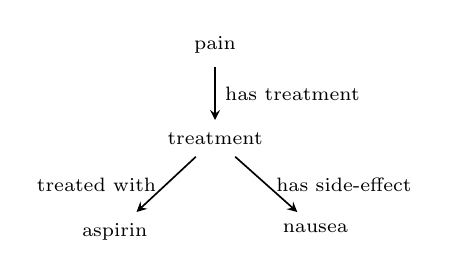
\begin{tikzpicture}[semithick, font = \scriptsize, draw = black, -stealth, shorten < = 1pt, shorten > = 1pt]
  \node (pain) {pain};
  \node (treatment) [below = 0.75cm of pain] {treatment};
  \node (aspirin) [below left = 0.75cm and 0cm of treatment] {aspirin};
  \node (nausea) [below right = 0.75cm and 0cm of treatment] {nausea};

  \draw (pain) -- node [midway, right] {has treatment} (treatment);
  \draw (treatment) -- node [midway, left] {treated with} (aspirin);
  \draw (treatment) -- node [midway, right] {has side-effect} (nausea);
\end{tikzpicture}

  \caption{The \textsc{treatment} node acts as mediator to represent a multi-ary relationship between \textsc{pain} and a treatment.}\label{fig:mediator}
\end{figure}

The problem with this is that a part of the link prediction task is to predict
\begin{enumerate*}
  \item whether a specific medical condition has a treatment and
  \item whether a specific drug is used for a treatment.
\end{enumerate*}
These tasks are clearly trivial.
Instead, a more interesting and realistic task is to predict
\begin{enumerate*}
  \item what drug is used for treating a specific medical condition and
  \item what medical conditions can be treated using a specific drug.
\end{enumerate*}

We believe that the absence of reverse and Cartesian product relations is the main explanation of the results from the domain-specific experiments in Section~\ref{sec:domain-specific}.
The dataset used in the experiment does not contain relations that form reverse or Cartesian product triples.

\subsection{Future Work}

In its nature, a \ac{kg} is of course a graph and thus exhibits many interesting properties that can be taken into consideration for link prediction.
However, graph embedding-based approaches for link prediction such as TransE, RotatE, and \ac{hake} only consider the triples in isolation when learning the embedding, and thus only learn the structure of the graph.
Immediately, it seems that properties and semantics of relations and entities in the \ac{kg} are lost in this process.
To address the link prediction problem effectively, future work should take into consideration not only the structure of the graph, but also the semantics of entities and their relations.
We think that one of the first steps to consider such semantics is to cluster entities into groups that share similar properties.
In\cite{Chen2019} an efficient approach for graph clustering is introduced.
Here, similarity between nodes is measured both by their structure and their attributes.
This clustering step is applied to star-schema heterogeneous graphs which are defined in the following way.

\begin{definition}[Star-schema heterogeneous graph]
  A heterogeneous graph is a 4-tuple $(V, E, \phi, \psi)$ where $V$ is a set of nodes, $E \subseteq V \times V$ is a set of edges, $\phi \colon V \rightarrow \mathcal{T}_V$ maps each $v \in V$ to a node type ${\mathcal{T}_V}_i \in \mathcal{T}_V$, and $\psi \colon E \rightarrow \mathcal{T}_E$ maps each $e \in E$ to an edge type ${\mathcal{T}_E}_i \in \mathcal{T}_E$.
\end{definition}

A heterogeneous graph is said to be on star-schema form if
\begin{enumerate*}
  \item node attributes are represented as nodes themselves, called attribute nodes, and
  \item nodes that share attributes are connected to the same attribute nodes.
\end{enumerate*}
Furthermore, non-attribute nodes are referred to as hub nodes, i.e.\ we have $\mathcal{T}_V = \{\text{hub}, \text{attribute}\}$.
In context of the medical domain, for instance, diseases and drugs can be hub nodes while symptoms, effects, and causes are attribute nodes.
\figurename~\ref{fig:heterogeneous-star-schema} illustrates the difference between a \enquote{regular} heterogeneous graph and a star-schema heterogeneous graph.
The $d_i$ hub nodes represent diseases and are connected to the $c_i$ and $s_i$ attributes nodes representing causes and symptoms.

\begin{figure}[ht]
  \centering\small
  \subfloat[Heterogeneous]{\centering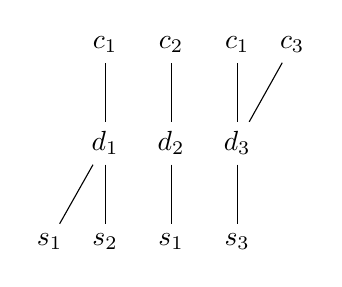
\begin{tikzpicture}[node distance = 0.75cm]
  \node (d1) {$d_1$};
  \node [below left = 0.75cm and 0.125cm of d1] (d1s1) {$s_1$};
  \node [below = of d1] (d1s2) {$s_2$};
  \node [above = of d1] (d1c1) {$c_1$};
  \draw [-] (d1) -- (d1s1);
  \draw [-] (d1) -- (d1s2);
  \draw [-] (d1) -- (d1c1);

  \node [right = 0.25cm of d1] (d2) {$d_2$};
  \node [above = of d2] (d2c2) {$c_2$};
  \node [below = of d2] (d2s1) {$s_1$};
  \draw [-] (d2) -- (d2c2);
  \draw [-] (d2) -- (d2s1);

  \node [right = 0.25cm of d2] (d3) {$d_3$};
  \node [above = of d3] (d3c1) {$c_1$};
  \node [above right = 0.75cm and 0.125cm of d3] (d3c3) {$c_3$};
  \node [below = of d3] (d3s3) {$s_3$};
  \draw [-] (d3) -- (d3c1);
  \draw [-] (d3) -- (d3c3);
  \draw [-] (d3) -- (d3s3);
\end{tikzpicture}
}\qquad
  \subfloat[Star-schema]{\centering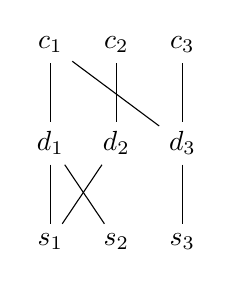
\begin{tikzpicture}[node distance = 0.75cm]
  \node (d1) {$d_1$};
  \node [right = 0.25cm of d1] (d2) {$d_2$};
  \node [right = 0.25cm of d2] (d3) {$d_3$};

  \node [below = of d1] (s1) {$s_1$};
  \node [below = of d2] (s2) {$s_2$};
  \node [below = of d3] (s3) {$s_3$};

  \node [above = of d1] (c1) {$c_1$};
  \node [above = of d2] (c2) {$c_2$};
  \node [above = of d3] (c3) {$c_3$};

  \draw [-] (d1) -- (s2);
  \draw [-] (d1) -- (s1);
  \draw [-] (d1) -- (c1);
  \draw [-] (d2) -- (c2);
  \draw [-] (d2) -- (s1);
  \draw [-] (d3) -- (s3);
  \draw [-] (d3) -- (c1);
  \draw [-] (d3) -- (c3);
\end{tikzpicture}
}
  \caption{The normalisation of the attributes in the left heterogeneous graph produces the star-schema graph on the right.}%
  \label{fig:heterogeneous-star-schema}
\end{figure}

It is clear that we can represent a \ac{kg} as a star-schema heterogeneous graph since it is a special case of a graph.
Since the star-schema structure is capable of capturing similarity both in terms of the properties of entities and how they are related, we think that it may help improving link prediction techniques.
Furthermore, most current \ac{kg} link prediction techniques expect the graph to be homogeneous\cite{Cai2018}.
As such, using star-schema heterogeneous graphs for future research can also uncover advantages and disadvantages of using heterogeneous graphs in this problem setting.

Another issue that can be addressed by avoiding graph embeddings for link prediction is flexibility and scalability.
A graph embedding is fixed to the \ac{kg} it has been learned on.
If we add new knowledge to a \ac{kg}, either entities or relations, the embedding must be re-computed.
This can become expensive and likely infeasible when the frequency of changes or the size of the \ac{kg} increases.
In connection with this, the embedding-based techniques also lack transparency when used for link prediction.
If the model predicts a given link, it is not immediately obvious why that link might exist.
Explainability is a not an issue that most \ac{kg} link prediction techniques currently try to address but it may be worth considering in future research since it is an increasingly important topic\cite{Gilpin2018}.
Similarity measures on graphs are more clear for humans since the specific attributes or nodes that explain the similarity can be pointed out and inspected.

Therefore, we propose that future work in the field of link prediction, and \ac{kg} refinement in general, should take similarity into account.
This can be done with star-schema heterogeneous graphs as a foundation since they offer a unified similarity measure that exhibits promising results.



\section{Conclusion}\label{sec:conclusion}

Representing \acp{kg} as low-dimensional vector embeddings has its computational advantages.
Querying existing knowledge is fast since arithmetic operations on embedded entities and relations act as translation from head entity to tail entity and vice versa.
The \ac{hake} technique, furthermore, has the advantages of being able to model hierarchical knowledge and complex relations.
However, the technique is not very precise and without a successful replication experiment, we doubt that the technique is flexible and scalable enough to be implemented in real-world use cases.
This argument is substantiated by the fact that performance on domain-specific data is significantly worse than on general-domain knowledge found in standard datasets.
We conclude that embedding technique might not be a suitable method for the link prediction problem in \acp{kg}.
Therefore, a deeper investigation into correct methods for the problem is necessary.
Any future solution to this problem should consider not only the structure of the graph, but also the semantics of entities and their relations, for it to work effectively.


\bibliographystyle{IEEEtran}
\bibliography{IEEEabrv, bibliography.bib}

\end{document}
